% Original vector reconstruction of source Fig.81.1, PDF329 / printed317.
% Counterclockwise external order: 1,2,3,4. Wavy-line arrows are momenta.
% The two internal momenta point left-to-right and bottom-to-top respectively;
% the opposite vertex always receives the negative of that assigned momentum.
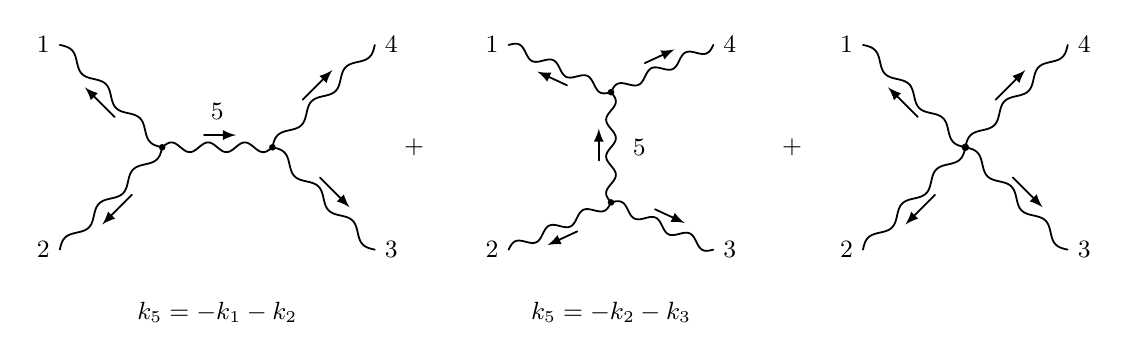
\begin{tikzpicture}[x=1mm,y=1mm,line width=.65pt,>=latex,
  line cap=round,line join=round,font=\fontsize{9}{11}\selectfont]
  % A short parallel arrow marks momentum without hiding the gluon wave.
  \def\sW#1#2#3{%
    \begin{scope}[shift={#1},rotate=#2]
      \draw plot[domain=0:1,samples=61]
        ({#3*\x},{.62*sin(1080*\x)});
      \draw[->] ({.38*#3},1.55)--({.67*#3},1.55);
    \end{scope}}
  \begin{scope}[shift={(22,0)}]
    \sW{(-7,0)}{135}{18.385}
    \sW{(-7,0)}{225}{18.385}
    \sW{(7,0)}{-45}{18.385}
    \sW{(7,0)}{45}{18.385}
    \sW{(-7,0)}{0}{14}
    \fill (-7,0) circle[radius=.42mm];
    \fill (7,0) circle[radius=.42mm];
    \node[above] at (0,2.2) {$5$};
    \node[left] at (-20,13) {$1$};
    \node[left] at (-20,-13) {$2$};
    \node[right] at (20,-13) {$3$};
    \node[right] at (20,13) {$4$};
    \node at (0,-21) {$k_5=-k_1-k_2$};
  \end{scope}
  \node at (47,0) {$+$};
  \begin{scope}[shift={(72,0)}]
    \sW{(0,7)}{155.224859}{14.317821}
    \sW{(0,7)}{24.775141}{14.317821}
    \sW{(0,-7)}{204.775141}{14.317821}
    \sW{(0,-7)}{-24.775141}{14.317821}
    \sW{(0,-7)}{90}{14}
    \fill (0,7) circle[radius=.42mm];
    \fill (0,-7) circle[radius=.42mm];
    \node[right] at (1.5,0) {$5$};
    \node[left] at (-13,13) {$1$};
    \node[left] at (-13,-13) {$2$};
    \node[right] at (13,-13) {$3$};
    \node[right] at (13,13) {$4$};
    \node at (0,-21) {$k_5=-k_2-k_3$};
  \end{scope}
  \node at (95,0) {$+$};
  \begin{scope}[shift={(117,0)}]
    \sW{(0,0)}{135}{18.385}
    \sW{(0,0)}{225}{18.385}
    \sW{(0,0)}{-45}{18.385}
    \sW{(0,0)}{45}{18.385}
    \fill (0,0) circle[radius=.48mm];
    \node[left] at (-13,13) {$1$};
    \node[left] at (-13,-13) {$2$};
    \node[right] at (13,-13) {$3$};
    \node[right] at (13,13) {$4$};
  \end{scope}
\end{tikzpicture}

